\documentclass[12pt,a4paper]{article}

% Packages
\usepackage{amsmath}
\usepackage{amsfonts}
\usepackage{amssymb}
\usepackage{graphicx}
\usepackage[margin=1in]{geometry}
\usepackage{enumitem}
\usepackage[hidelinks]{hyperref}

% Title
\title{Homework Report for Computer Vision}
\author{Yu Xiang, Luo}
\date{\today}

\begin{document}

\maketitle

% Introduction
\[
	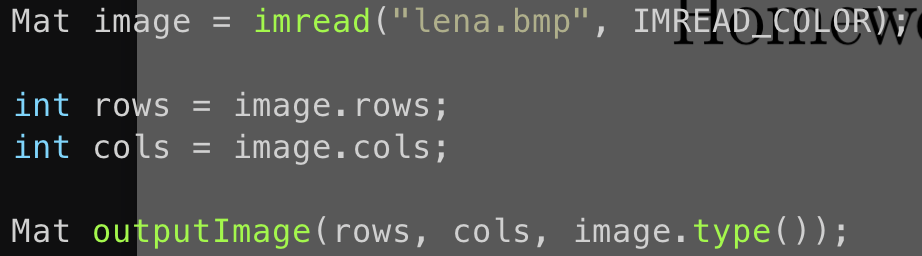
\includegraphics[width=0.9\textwidth]{./image/p0.png}
\]
\[
	\text{First, we have to read the bmp file and create the output image.}
\]
\[
	\href{https://github.com/YuXiangLo/Computer-Vision}{\text{Complete Code}}
\]
\section*{Part 1}
\begin{enumerate}[label=(\alph*)]
	\item Simply reverse the X-axis index can solve this problem.\\ 
		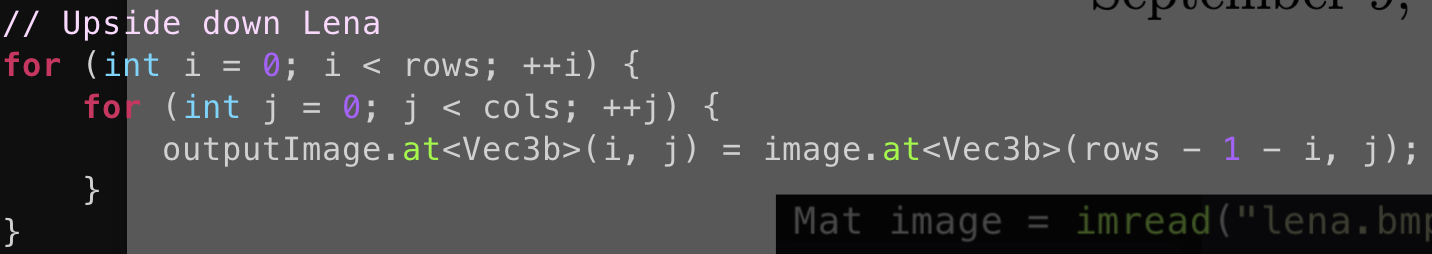
\includegraphics[width=0.9\textwidth]{image/p1.png}
	\item Simply reverse the Y-axis index can solve this problem.\\
		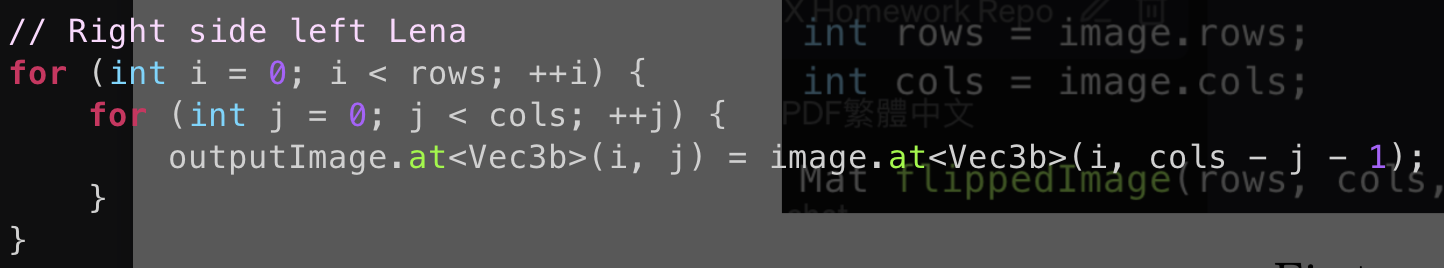
\includegraphics[width=0.9\textwidth]{image/p2.png}
	\item Simultaneously reverse X-axis and Y-axis can solve this problem.\\
		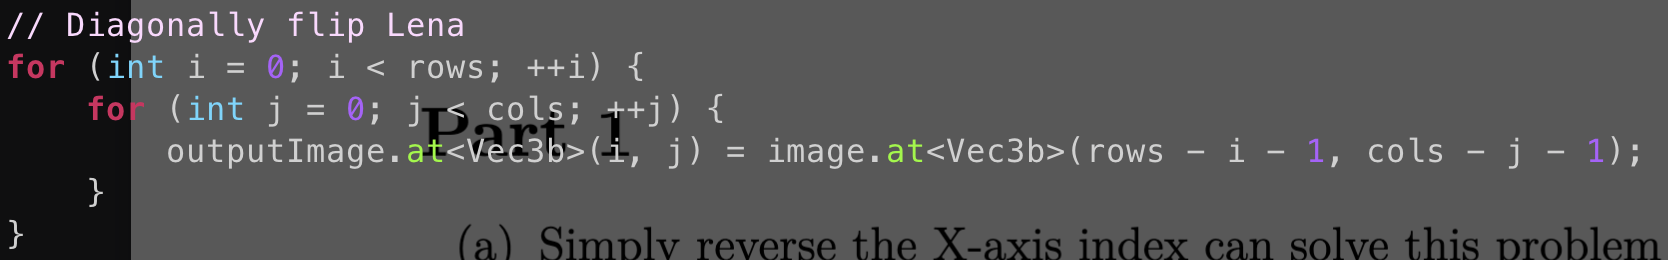
\includegraphics[width=0.9\textwidth]{image/p3.png}
\end{enumerate}

\section*{Part 2}
\begin{enumerate}[label=(\alph*), resume]
	\item In this case, we need to find the center, calculate the radians of the degree of 45, and operate the image using the transformation matrix.\\
	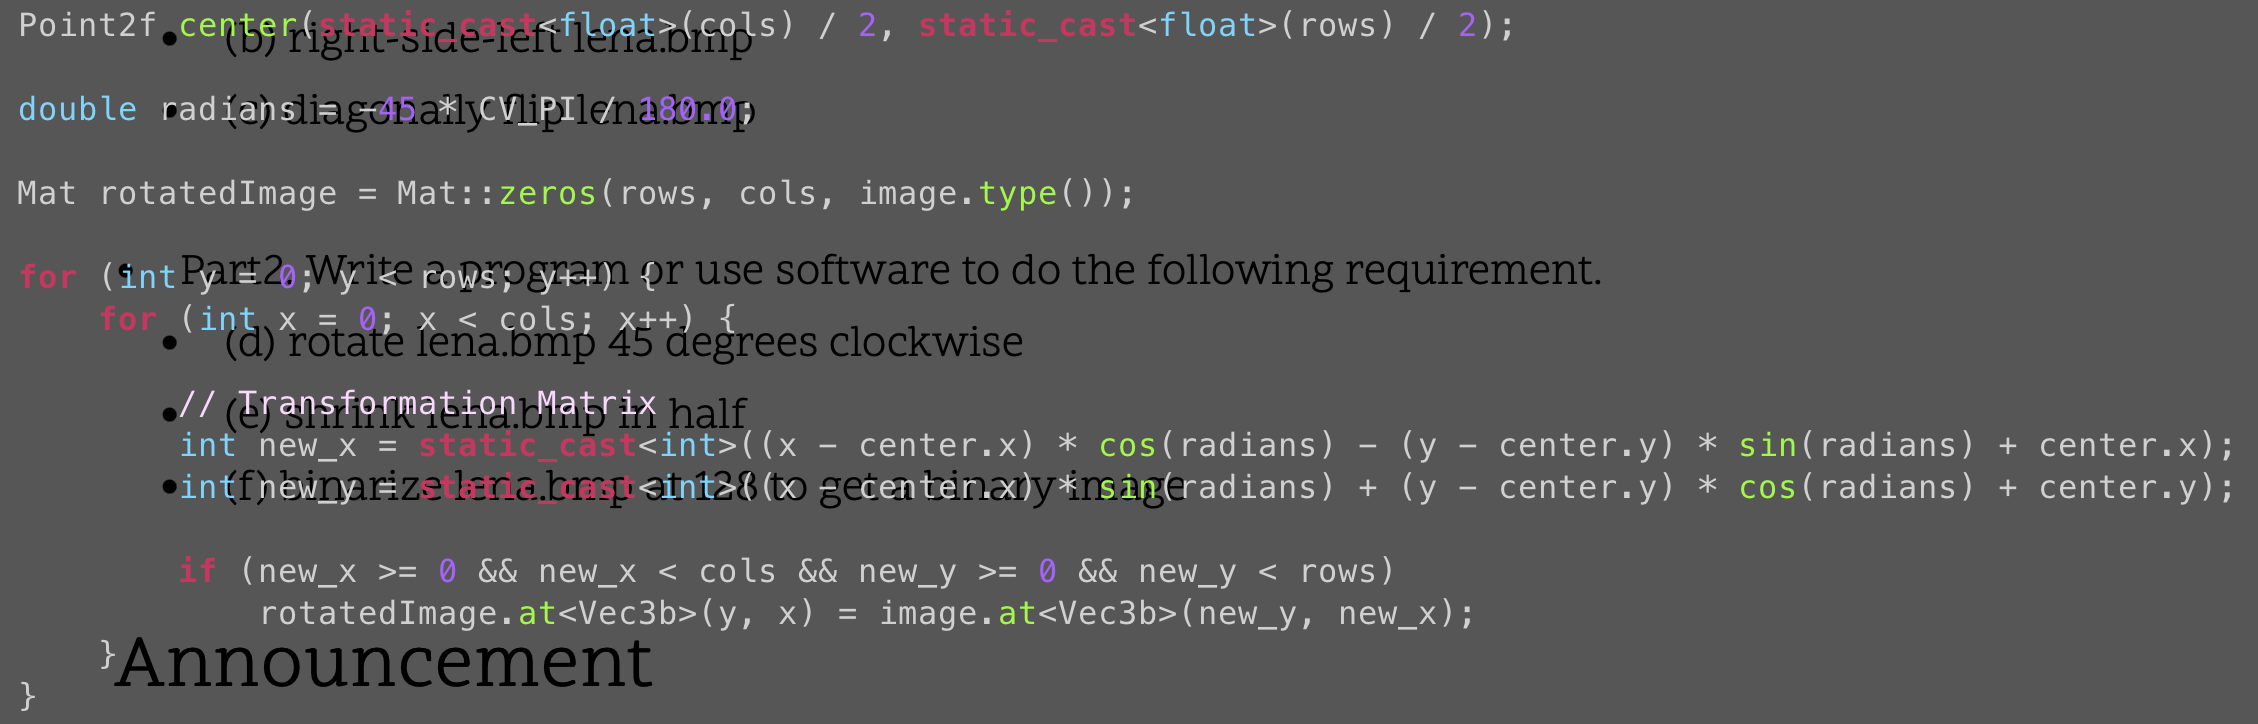
\includegraphics[width=0.9\textwidth]{image/p4.png}
	\item Just call the function in opencv can solve this easily.\\
		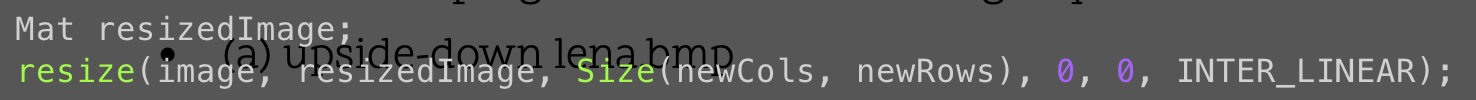
\includegraphics[width=0.9\textwidth]{image/p5.png}
	\item Call the function in opencv.\\
		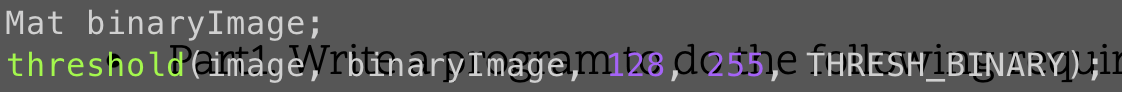
\includegraphics[width=0.9\textwidth]{image/p6.png}
\end{enumerate}

\section*{All the output Lena}
\begin{enumerate}[label=(\alph*)]
	\item Upside down Lena\\ 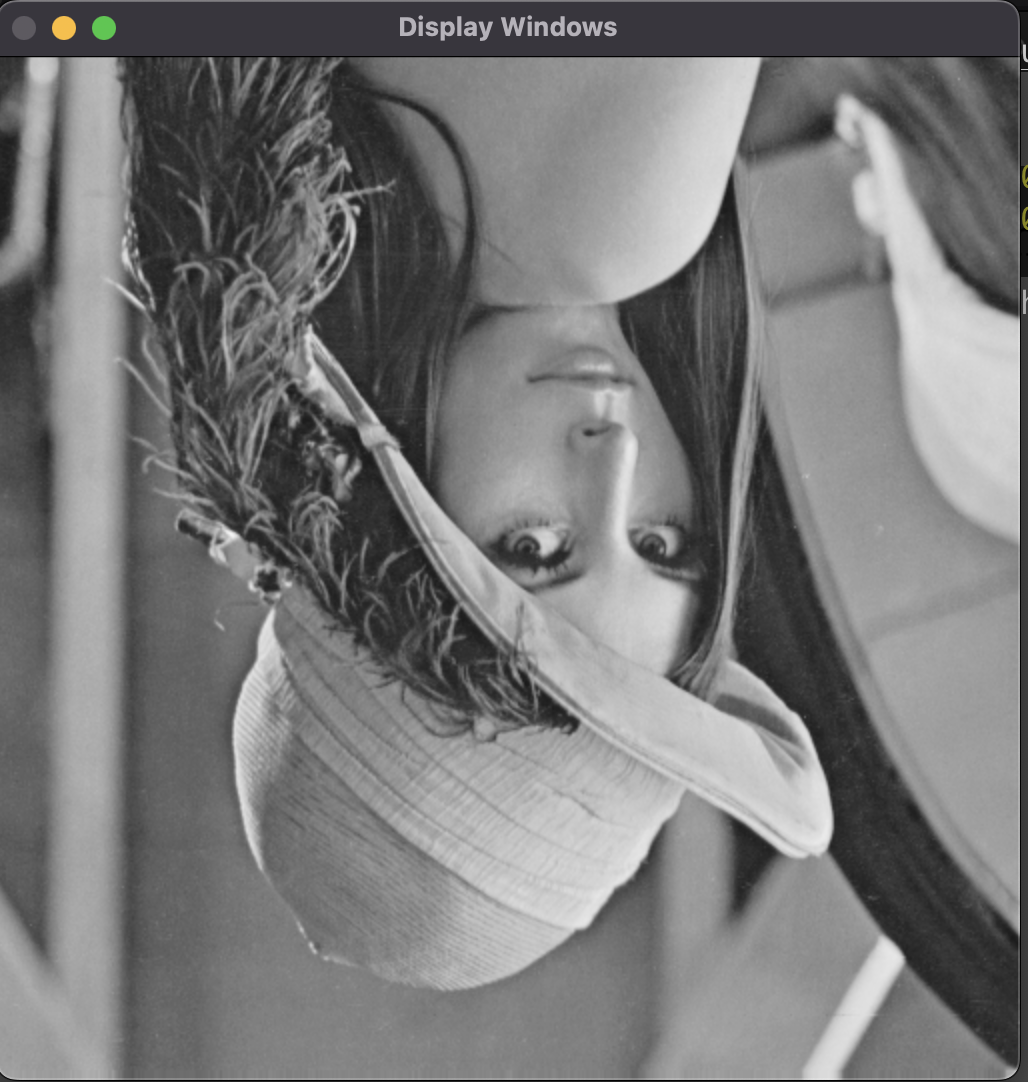
\includegraphics[width=0.3\textwidth]{image/p1o.png}
	\item Right side left Lena\\ 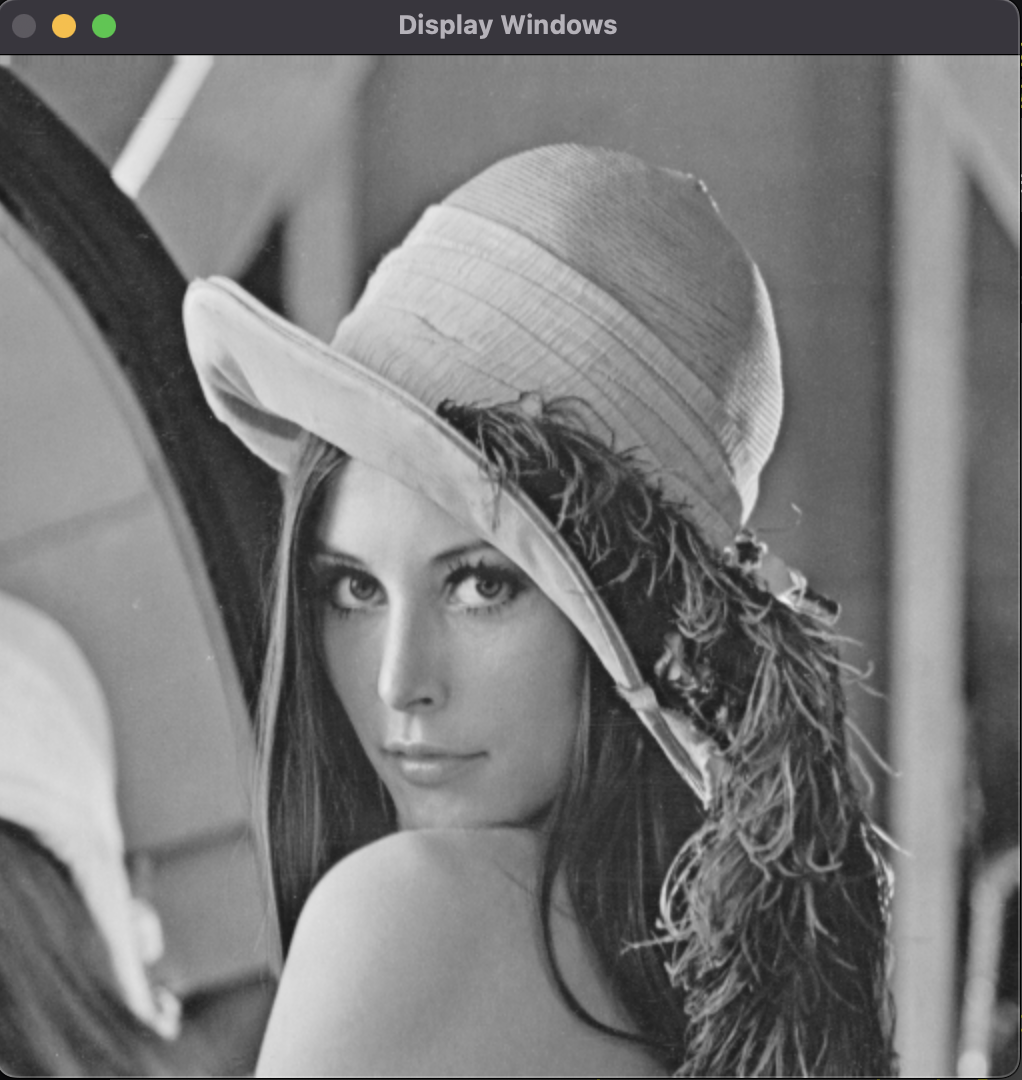
\includegraphics[width=0.3\textwidth]{image/p2o.png}
	\item Diagonally flip Lena\\ 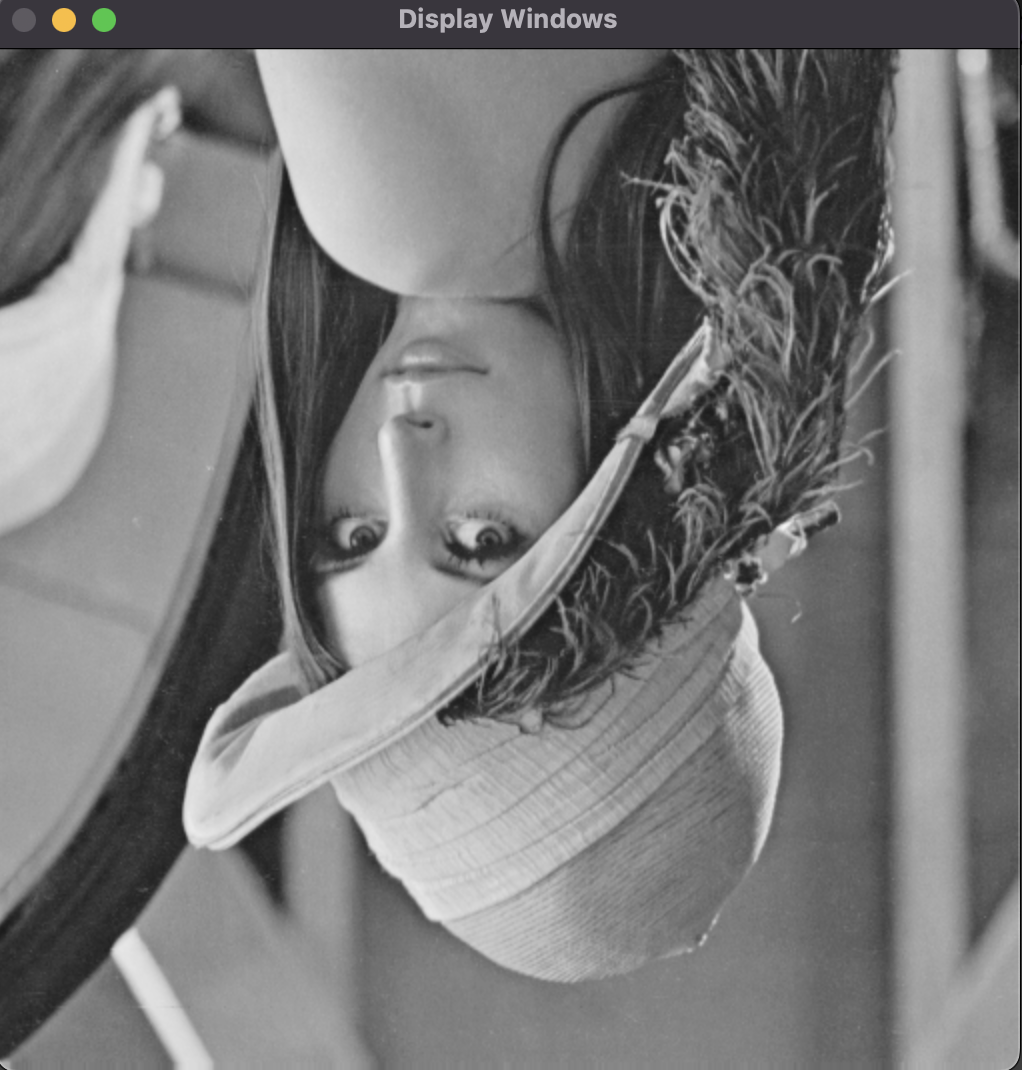
\includegraphics[width=0.3\textwidth]{image/p3o.png}
	\item Rotate Lena\\ 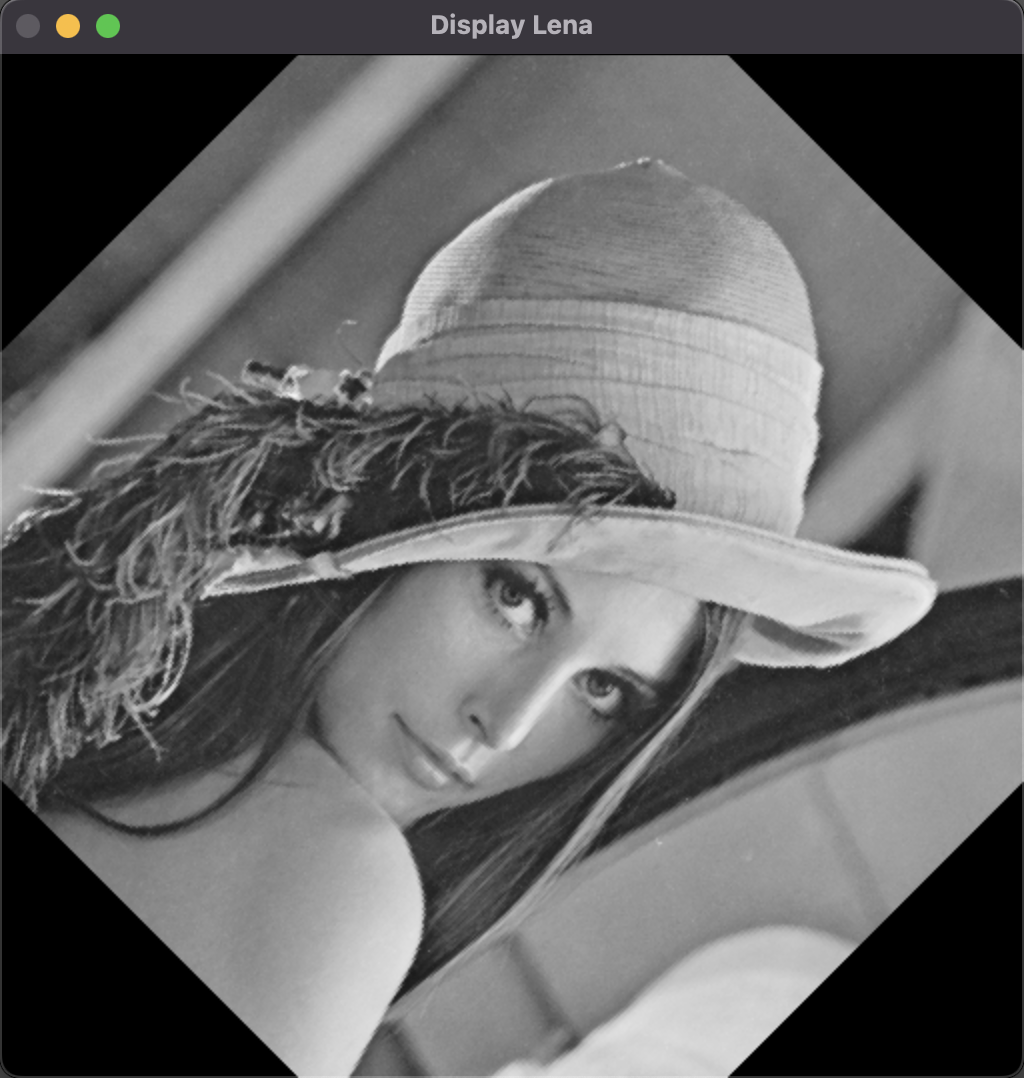
\includegraphics[width=0.3\textwidth]{image/p4o.png}
	\item Shrink Lena\\ 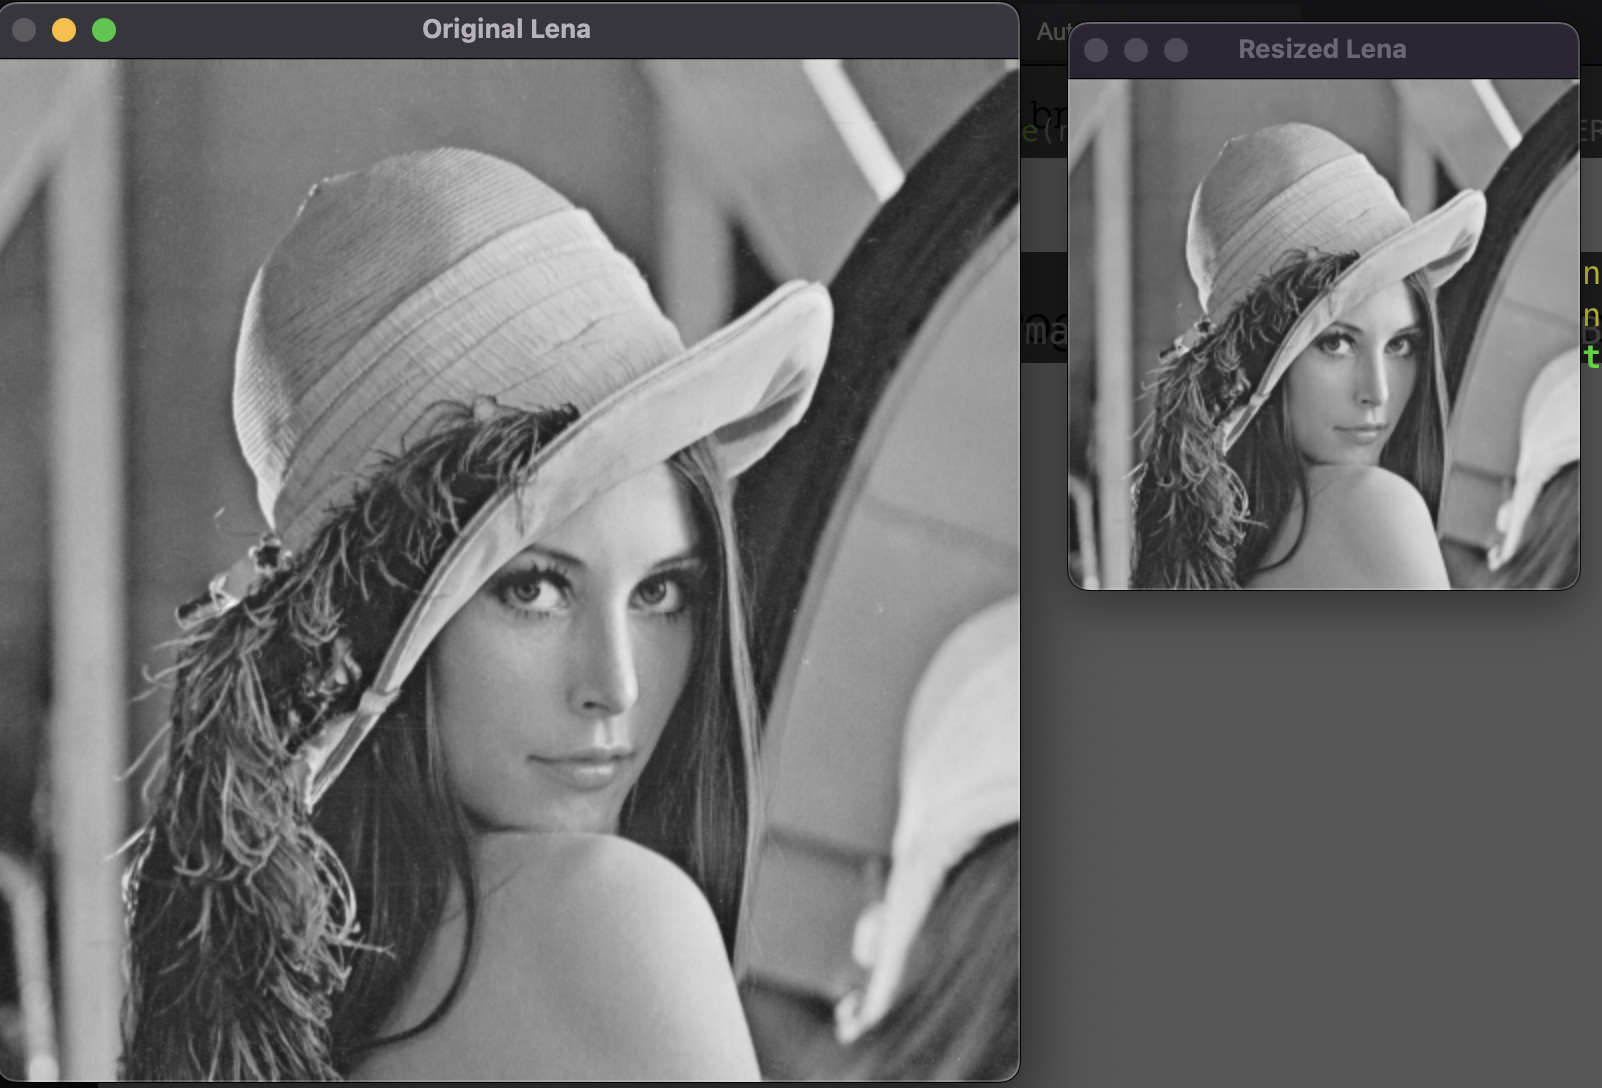
\includegraphics[width=0.3\textwidth]{image/p5o.png}
	\item Binarized Lena\\ 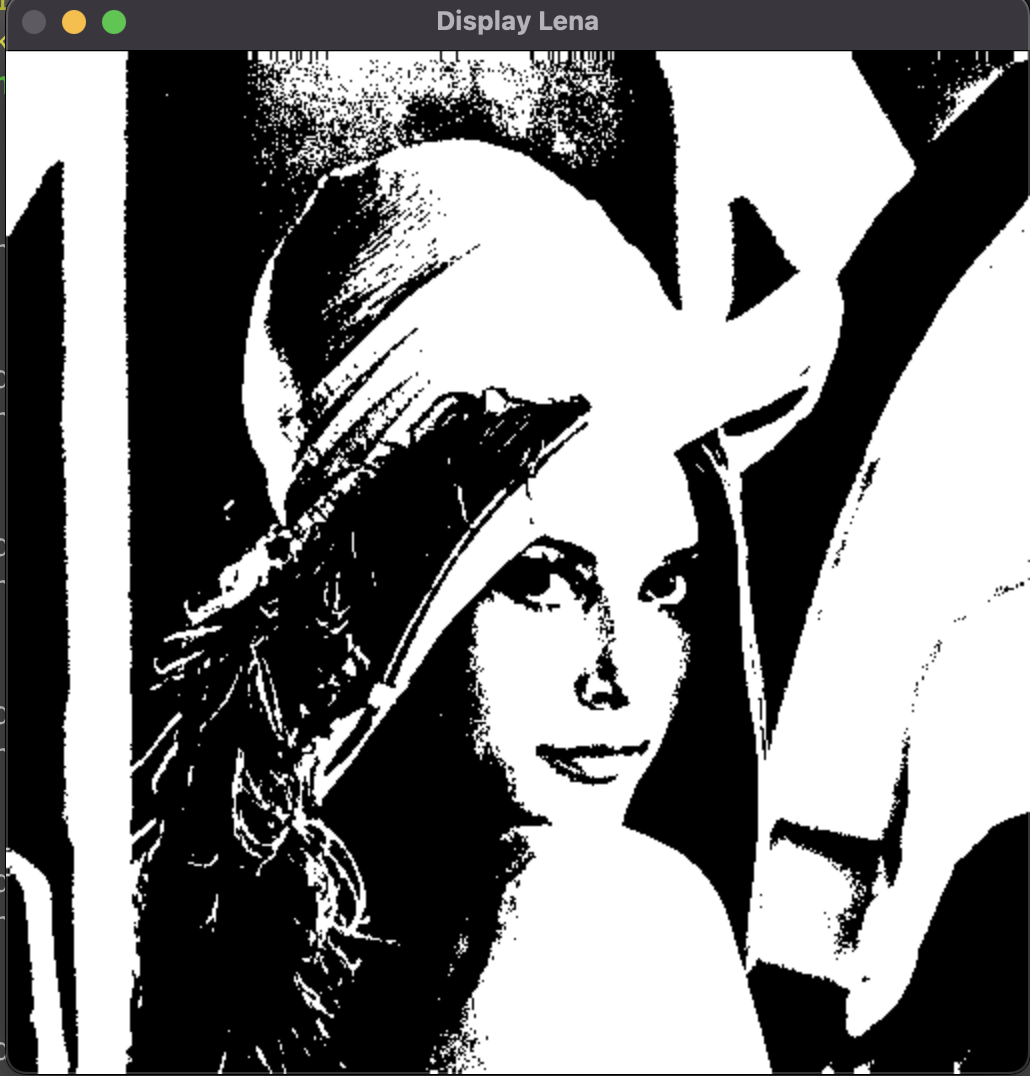
\includegraphics[width=0.3\textwidth]{image/p6o.png}
\end{enumerate}


\end{document}

